 \documentclass[a4paper, 10pt, notitlepage]{article}

\usepackage[english]{babel}
\usepackage[latin1]{inputenc}
\usepackage{amsmath}
\usepackage{amsfonts}
\usepackage{graphicx}
\usepackage{url}
\usepackage{layaureo}
\usepackage{wrapfig}
\usepackage[font=footnotesize]{caption}
\usepackage[font=footnotesize]{subcaption}
\usepackage[style=numeric, sorting=none, backend=biber]{biblatex}

\addbibresource{reference.bib}

\author{G. Bertoli \and A. Shcherbakova \and E. Valdes}
\title{Readiness of the PingaTube of the Group~5 Collaboration}
\date{2 November 2015}

\graphicspath{{./images/}}

\newcommand{\ud}{\mathrm{d}}

\begin{document}
\maketitle

\begin{abstract}
  The PingaTube is the proportional counter of the Group 5 collaboration.
%%% Local Variables:
%%% mode: latex
%%% TeX-master: "prop_counter"
%%% End:

\end{abstract}

\section{Introduction}
\label{sec:intro}
Insert introduction
%%% Local Variables:
%%% mode: latex
%%% TeX-master: "prop_counter"
%%% End:


\section{Theoretical overview}
\label{sec:theory}
Insert theory
%%% Local Variables:
%%% mode: latex
%%% TeX-master: "prop_counter"
%%% End:


\section{Building of the proportional counters}
\label{sec:build-prop-count}
\subsection{Materials for the PingaTube}
\label{sec:materials_pingatube}
In order to build the PingaTube detector the following parts were used:
\begin{itemize}
\item a cathod consisting in a aluminium tube (l = 146.5 mm, d$_{inner}$ = 20.63
  mm, d$_{outer}$ = 22.9 mm, d$_{window}$ = 9.2 mm)
\item an anode consisting in a Cu/Be wire (d = 0.025 mm)
\item two bras tubes to prevent gas multiplication at the end of the active
  volume (d = 1 mm, l$_{1}$ = 40.64 mm and l$_{1}$ = 42.72 mm)
\item insulating endcaps
\item P-10 gas Argon (90\%)/CH$_{4}$ (10\%)
\item gas tubes in order to convey the gas (d = 2.1 mm)
\item High voltage (HV) connector in order to supply high voltage to the anode
\item a ground cable in order to connect the cathode
\item O-ring wire connector
\item electric fastenning belt
\item Ultrasound bath with 10/90 Isopropanol/Water
\item Lab tools (Caliper (precition = 1/100 mm), Needle, Gloves, Files, Drill,
  Saw, Microscope, Oscilloscope, etc) and consumables (Soldering flux, aluminium
  tape, epoxy glue, etc)
\end{itemize}

\subsection{Design and Assembly of the PingaTube}
\label{sec:design_and_assembly_beercan}
The main target was to be able to design, build and use in a real data taking
experiment a proportional counter detector using every day objects. Most of the
materials were provided and hence creatively assembling the detector was the
main task. Due to safety regulations some steps, mostly cutting and drilling,
were handled by the instructors.

The bras tubes were sanded at the extremities to avoid sparks that could damage
the anode and, using a microscope, it was verified that no significant notches
were present. Any residue of grease on any of the internal parts could cause
dishomogeneities of the electric field and thus compromise the energy
resolution. In order to prevent this, all the parts were cleaned in an
ultrasonic bath of isopropanol/water mixture.

The thickness of the cathode tube was enough to stop the radiation from the
weaker source of Fe55 thus a small window, that was later covered with a thin
aluminum foil, was opened approximately in the middle of it. Holes were drilled
on plastic endcaps to flush the gas in the active volume and to fit the brass
tubes.

In the assembly phase, the Cu/Be wire was let through the endcaps, the cathode
and the bras tubes which were then put in place in the endcaps. It was then
soldered to a HV connector together with one of the bras tubes on one side and
to the ground on the other. Everything was then sealed using a bi-component
epoxy glue and the cathode was connected to ground.

After the assembly process the P-10 gas was flushed into the detector in order
to extract as much O$_2$ as possible. The main reason for this is that O$_2$ is
a quenching gas that absorbs the avalanche electrons. Leakages of gas from the
detector tube was checked with a flowmeter. The volume of the aluminum tube is
$\approx$ 49~cm$^3$
% \emph{Volume of the tube}, Volume of the tube
% \begin{equation}
%   \label{eq:tube_volume}
%   V=\frac{\pi L^2}{4} =14.65*3.14*2.06324*2.06324=48,96 cm^3
% \end{equation}
With a flow 10 ml/min = 600 cm$^3$/h content of the volume changes ~10 times per
hour. The variation of O$_{2}$ concentration with time is shown on
Figure~\ref{fig:ppm}, it can be seen that the sealing of the detector was
good.
% Units of x-axis are ppm = 1,000,000 m$_{c}$ / m$_{s}$, where m$_{c}$ =
% mass of component (argon/methane mix, kg) m$_{s}$ = mass of solution (oxygen,
% kg).
\begin{figure}[!h]
  \centering
  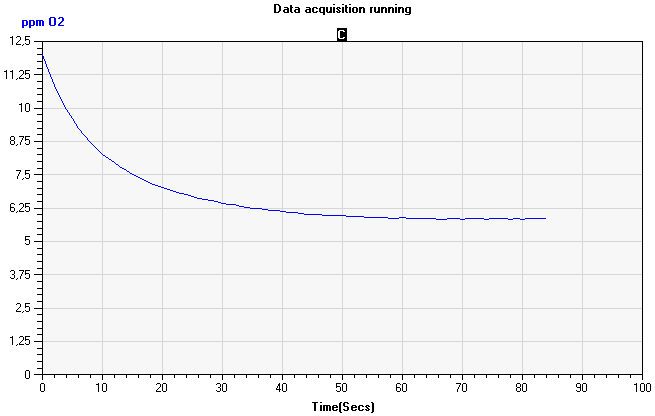
\includegraphics[width=.5\linewidth]{ppm}
  \caption{Variation of O$_2$ concentration as function of time}
  \label{fig:ppm}
\end{figure}

Some problems which were fixed:
\begin{itemize}
\item one of the gas tubes did were not inserted properly which caused gas
  leaking, The problem was sucessfuly fixed afterwards by removing and
  reinserting it properly.  This caused a lot of delay due to the time that the
  glue takes to drying besides the fact that it was needed to reflux the gas on
  the detector.
\item One of the brass tubes slipped inside of the aluminum tube. The issue
  was sorted out on time before the glue dried without any further problem.
\end{itemize}

\subsection{Materials for the BeerCan}
\label{sec:materials_beercan}
In order to build the BeerCan detector the following parts were used:
\begin{itemize}
\item a catode consisting in a beer can (l = 146.5 mm, d$_{inner}$ = 64.0 mm,
  d$_{thickness}$ = 0.2 mm)
\item an anode consisting in a Cu/Be wire (d = 0.075 mm)
\item two bras tubes. (d = 1 mm, l$_{1}$ = 40.64 mm and l$_{1}$ = 42.72 mm)
\item guide in order to protect the brass tubes of touching the can (d = 3.21
  mm)
\item plastic endcaps
\item gas tubes in order to convey the gas (d = 2.1 mm)
\item HV connector in order to supply high voltage to the anode
\item a ground cable in order to connect the cathode.
\item P10 gas Argon (90\%)/CH$_{4}$ (10\%)
\item Ultrasound bath with 10/90 Isopropanol/Water
\item Lab tools (Caliper (precition = 1/100 mm), Needle, Gloves, Files, Drill,
  Saw, Microscope, Oscilloscope, etc) and consumables (Soldering flux, aluminium
  tape, epoxy glue, etc)
\end{itemize}

\subsection{Design and Assembly of the BeerCan}
\label{sec:design_and_assembly_beercan}
The building and assembly was very similar to the description on the PingaTube
detector with the mechanical differences imposed by the beer can geometry.
Again most of the materials were provided and hence creatively assembling the
detector was the main task. After the assembly process the P-10 gas was flushed
into the detector and the flowmeter was used for detecting gas leakages.  Some
differences in the assembly of the BeerCan detector compared to the PingaTube
detector were:
\begin{itemize}
\item Necesity of scratching inner and outer surfaces of the beer can so the
  non-conductive cover was removed.
\item Use of 0.075 mm brass tubes for easier manipulation and insertion of the
  Cu/Be wire.
\end{itemize}
The brass tubes had a diameter of 5.5 mm. The length was chosen so that their
end was at a distance of 3~cm from the center of the can. Further, the diameter
of the gas tubes was 2.86~mm and the length of banana plug was 67~mm.
% Volume of the beercan tube: \emph{Volume of the tube}, Volume of the tube
% \begin{equation}
%   \label{eq:tube_volume}
%   V=\frac{\pi L^2}{4} =14.65*3.14*6.40*6.40=471,05 cm^3
% \end{equation}
With a flow 10 ml/min = 600 cm$^3$/h content of the volume changes ~10 times per
hour.
Some problems that were solved:
\begin{itemize}
\item There was gas leaking in the endcaps, they were sealed by using the epoxy
  glue.
\item The Cu/Be wire got loose while trying to solder it to one of the bras
  tubes which might have caused the detector to have an extremely poor signal
  and was not possible to use it for data taking. There was not enough time for fixing this
  issue due to the lack of time and materials.
\end{itemize}
%%% Local Variables:
%%% mode: latex
%%% TeX-master: "prop_counter"
%%% End:


\section{Experimental setup}
\label{sec:setup}
\subsection{Building of the "PingaTube" detector}
\label{sec:building_pingatube}

\subsubsection{Materials for the PingaTube}
\label{sec:materials_pingatube}
In order to build the PingaTube detector the following parts were used:
\begin{itemize}
\item a cathod consisting in a aluminium tube (l = 146.5 mm, d$_{inner}$ = 20.63
  mm, d$_{outer}$ = 22.9 mm, d$_{window}$ = 9.2 mm)
\item an anode consisting in a Cu/Be wire (d = 0.025 mm)
\item two bras tubes to prevent gas multiplication at the end of the active
  volume (d = 1 mm, l$_{1}$ = 40.64 mm and l$_{1}$ = 42.72 mm)
\item insulating endcaps
\item P-10 gas Argon (90\%)/CH$_{4}$ (10\%)
\item gas tubes in order to convey the gas (d = 2.1 mm)
\item High voltage (HV) connector in order to supply high voltage to the anode
\item a ground cable in order to connect the cathode
\item O-ring wire connector
\item electric fastenning belt
\item Ultrasound bath with 10/90 Isopropanol/Water
\item Lab tools (Caliper (precition = 1/100 mm), Needle, Gloves, Files, Drill,
  Saw, Microscope, Oscilloscope, etc) and consumables (Soldering flux, aluminium
  tape, epoxy glue, etc)
\end{itemize}

\subsubsection{Design and Assembly}
\label{sec:design_and_assembly_beercan}
The main target was to be able to design, build and use in a real data taking
experiment a proportional counter detector using every day objects. Most of the
materials were provided and hence creatively assembling the detector was the
main task. Due to safety regulations some steps, mostly cutting and drilling,
were handled by the instructors.

The bras tubes were sanded at the extremities to avoid sparks that could damage
the anode and, using a microscope, it was verified that no significant notches
were present. Any residue of grease on any of the internal parts could cause
dishomogeneities of the electric field and thus compromise the energy
resolution. In order to prevent this, all the parts were cleaned in an
ultrasonic bath of isopropanol/water mixture.

The thickness of the cathode tube was enough to stop the radiation from the
weaker source of Fe55 thus a small window, that was later covered with a thin
aluminum foil, was opened approximately in the middle of it.

The Cu/Be wire was soldered to the HV connector and glued to the end caps. In
order to fix and seal the chamber the end caps were glued with a two component
epoxy glue.  The Cu/Be wire was inserted thru two brass tubes in both the
extremes of the chamber in order to ensure as uniform field as possible.  A
window in a form of circular hole was drilled around the middle part of the
chamber. The end caps have holes to provide access for gas tubes, they were
glued in both sides with the epoxy glue.  The Cu/Be wire and the pipe were
connected and soldered the high voltage connector as anode and ground
respectively. A part of the aluminum tube was polished to create space for
grounding and that surface was covered with copper tape for providing better
contact.  Given that the Cu/Be is toxic gloves were required for handling it.
Additionally the wire easily bends increasing the risk of it being break. The
wire was soldered to the extremes of the brass tubes already mounted in the end
caps. All was sealed with the epoxy glue afterwards.

After the assembly process the P10 gas was flushed into the detector in order to
extract as much O$_2$ as possible. The main reason of this is O$_2$ is a
quenching gas that absorbs the avalanche electrons.  Presence of leakages of gas
from the detector tube was checked with a flowmeter. Volume of the aluminum
tube: \emph{Volume of the tube}, Volume of the tube
\begin{equation}
  \label{eq:tube_volume}
  V=\frac{\pi L^2}{4} =14.65*3.14*2.06324*2.06324=48,96 cm^3
\end{equation}
With a flow 10 ml/min = 600 cm$^3$/h content of the volume changes ~10 times per
hour. The variation of O$_{2}$ concentration with time is shown on Fig.  Units
of x-axis are ppm = 1,000,000 m$_{c}$ / m$_{s}$, where m$_{c}$ = mass of
component (argon/methane mix, kg) m$_{s}$ = mass of solution (oxygen, kg).  Some
failures which were fixed were:
\begin{itemize}
\item one of the gas tubes did were not interted properly which caused gas
  leaking, The problem was sucessfuly fixed afterwards by removing and
  reinserting it properly.  This caused a lot of delay due to the time that the
  glue delays on drying besides the fact that it was needed to reflux the gas on
  the detector.
\item There were some gas leakages that were sorted out propperly by glue
  sealing the positions in which the floweter detector establish the gas
  leakages.
\item One of the brass tubes went loose inside of the aluminium tube. The issue
  was sorted out on time before the glu dried without any further problem.
\end{itemize}

\subsection{Building of the "BeerCan" detector}
\label{sec:building_beercan}

\subsubsection{Materials for the BeerCan}
\label{sec:materials_beercan}
In order to build the "BeerCan" detector the following parts were used:
\begin{itemize}
\item a catode consisting in a beer can (l = 146.5 mm, d$_{inner}$ = 64.0 mm,
  d$_{thickness}$ = 0.2 mm)
\item an anode consisting in a Cu/Be wire as the anode (d = 0.075 mm)
\item two brass tubes. (d = 1 mm, l$_{1}$ = 40.64 mm and l$_{1}$ = 42.72 mm)
\item guide in order to protect the brass tubes of touching the can (d = 3.21
  mm)
\item bushing
\item plastic endcaps
\item gas tubes in order to flux the gas (d = 2.1 mm)
\item HV connector in order to supply high voltage to the anode
\item a ground cable in order to connect the cathode.
\item P10 gas Argon (90\%)/CH$_{4}$ (10\%)
\item Ultrasound bath with 10/90 Isopropanol/Water
\item Lab tools (Caliper (precition = 1/100 mm), Needle, Gloves, Files, Drill,
  Saw, Microscope, Oscilloscope, etc) and consumables (Soldering flux, aluminium
  tape, epoxy glue, etc)
\end{itemize}

\subsubsection{Design and Assembly of the BeerCan}
\label{sec:design_and_assembly_beercan}
The design was intended for using a beer can as gas chamber detector. The
building and assembly was very similar to the description on the PingaTube
detector with the mechanical differences imposed by the beer can geometry.
Again most of the materials were provided and hence creatively assembling the
detector was the main task. After the assembly process the P10 gas was flushed
into the detector and the flowmeter was used for detecting gas leakages.  Some
differences in the assembly of the BeerCan detector compared to the PingaTube
detector were:
\begin{itemize}
\item Necesity of scratching inner and outer surfaces of the beer can so the
  nonconductive cover was removed.
\item Use of 0.075 mm brass tubes for easier manipulation and insertion of the
  Cu/Be wire.
\end{itemize}
The brass tubes had a diameter of 5.5 mm. The length was chosen so that their
end is at a distance of 3 cm from the center of the can. Further, the diameter
of the gas tubes was 2.86 mm and the length of banana plug was 67 mm.
Volume of the beercan tube: \emph{Volume of the tube}, Volume of the tube
\begin{equation}
  \label{eq:tube_volume}
  V=\frac{\pi L^2}{4} =14.65*3.14*6.40*6.40=471,05 cm^3
\end{equation}
With a flow 10 ml/min = 600 cm$^3$/h content of the volume changes ~10 times per
hour. The variation of O$_{2}$ concentration with time is shown on Fig. Units of
x-axis are ppm = 1,000,000 m$_{c}$ / m$_{s}$, where m$_{c}$ = mass of component
(argon/methane mix, kg) m$_{s}$ = mass of solution (oxygen, kg)

Some failures:
\begin{itemize}
\item There was gas leaking in the endcaps, they were sealed by using the epoxy
  gum and covering all the leaking points detected.
\item The Cu/Be wire got blended and a little bit loose while trying to solder
  it to the one of the brass tubes which might have cause the detector to have
  an extremely poor signal hence it was considered a failure. There was not
  enough time for fixing this issue since it practically would have taken the
  dissasembly of the whole detector.
\end{itemize}

\subsection{Measurement apparatus}
\label{sec:meas-appar}
Figure~\ref{fig:exp_setup} shows a schematic view of the setup used for the
calibration of the detector and data taking. The signal from the detector at
first pass trough a pre-amplifier, this has a capacitance of 1~pF and is
connected to a high voltage power supply (HVPS) so that the input voltage is
directly proportional to the charge generated in the detector through the well
know formula\autocite{Knoll:RadMeasurement}
\begin{equation}
  \label{eq:capacitance}
  Q = CV.
\end{equation}
The pre-amplifier is then connected to a spectrum amplifier with adjustable gain
and a pulse generator. From the spectrum amplifier the signal was sent to an
oscilloscope for online monitoring and adjustments and to a multi-channel
analyzer (MCA) that was connected to a computer to record the data.
\begin{figure}[!h]
  \centering
  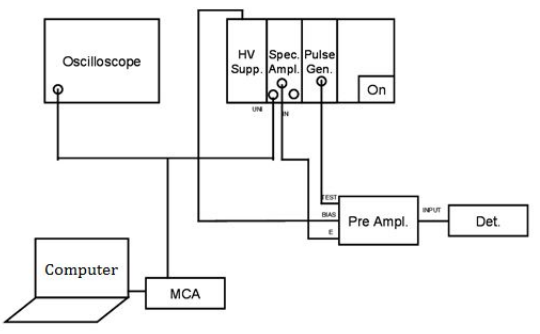
\includegraphics[width=.5\linewidth]{experimental_setup}
  \caption{Schema of the experimental setup}
  \label{fig:exp_setup}
\end{figure}

\subsection{Calibration}
\label{sec:calibration}
In order to calibrate the detector the pulse generator was used to injected in
the pre-amplifier a known pulse. The oscilloscope was used to read the pulse
voltage that multiplied by the pre-amplifier capacitance gives the collected
charge as described in Section~\ref{sec:meas-appar}. The distribution on the MCA
was fitted with a Gaussian using the data taking software, the mean value is
then associated to a charge and the standard deviation used as uncertainty. This
procedure was performed for a set of input voltages and, due to time
restrictions, only for a gain value of 100. Figure~\ref{fig:calibration_fit}
shows the calculated collected charge as a function of the MCA channel number
with a linear fit superimposed. Figure~\ref{fig:calibration_raw} shows the
counts as a function of the MCA channel number.
\begin{figure}[!h]
  \centering
  \begin{subfigure}[t]{.48\linewidth}
    \includegraphics[width=\linewidth]{calibration_fit}
    \caption{Collected charge as a function of the multi-channel number}
    \label{fig:calibration_fit}
  \end{subfigure}
  \begin{subfigure}[t]{.48\linewidth}
    \includegraphics[width=\linewidth]{calibration_raw}
    \caption{Counts as a function of the multi-channel number}
    \label{fig:calibration_raw}
  \end{subfigure}
  \caption{}
  \label{fig:calibration}
\end{figure}
%%% Local Variables:
%%% mode: latex
%%% TeX-master: "prop_counter"
%%% End:


\section{Results}
\label{sec:results}
\subsection{Calibration}
In order to calibrate the detector a know voltage was
\label{sec:calibration}
\begin{figure}[!h]
  \centering
  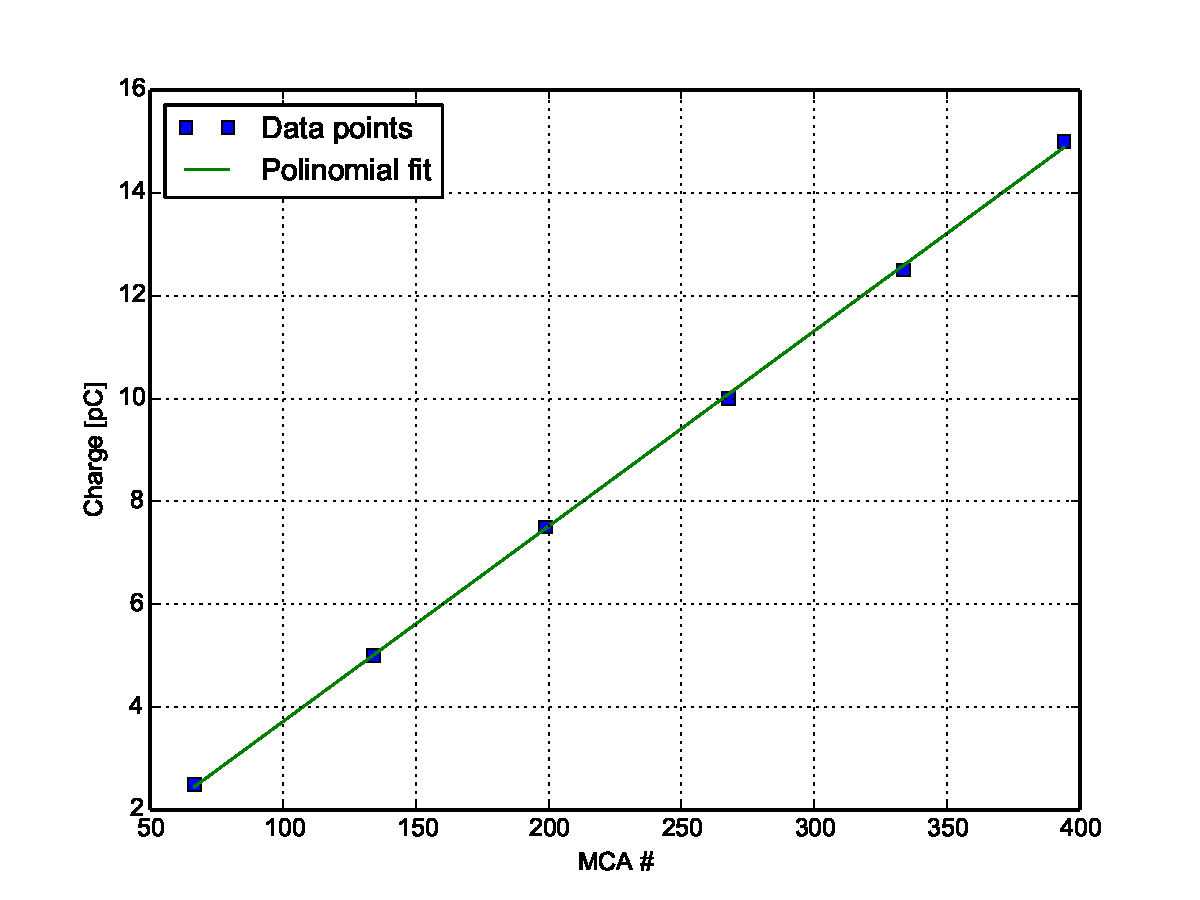
\includegraphics[width=.5\linewidth]{calibration}
  \caption{Collected charge as a function of the multi-channel number}
  \label{fig:calibration}
\end{figure}
\subsection{Errors}


The relationship between the HV:

\begin{equation}
  U_{HV(U_{ref})} = \alpha U_{ref} + \beta
\end{equation}

from where we can get the error as:

\begin{equation}
  \delta U_{HV(U_{ref})} = \sqrt{ (\delta \alpha  U_{ref})^2 + (\delta \beta)^2 + (\alpha \delta U_{ref})^2 }
\end{equation}

The charge collected in the anode was obtained feeding the input of the preamplifier with a square pulse and measuring the MCA response.

\begin{equation}
  Q = C U_{pulse (N)} 
\end{equation}

Where Q is the charge collected, the C capacitance and N is the multichannel analyzer response that depends lineary on the gain chosen.

\begin{equation}
  U_{pulse (N)}= C\alpha_G N_G + \beta_G
\end{equation}

Hence the error for Q would be:

\begin{equation}
  \delta Q = \sqrt{(\delta CU_p )^2 + (C \sqrt{(N\delta \alpha)^2+(\delta \beta)^2} )^2 + (C\alpha \delta N)^2}
\end{equation}

On the resolution side most errors treated and obtained from the Gaussian distribution

\begin{equation}
  \delta R = \sqrt{(\frac{\delta \sigma,}{\sigma})^2 + (\frac{\delta \mu}{\mu})^2}
\end{equation}



%%% Local Variables:
%%% mode: latex
%%% TeX-master: "prop_counter"
%%% End:


\section{Conclustions}
\label{sec:conclusions}
Insert conclusions.
%%% Local Variables:
%%% mode: latex
%%% TeX-master: "prop_counter"
%%% End:

During the lab two proportional counters were built one using a piece of a common aluminum tube and one using a common empty beer can. 
Both detectors were assembled and filed with an Ar-CH$_4$ mixture and a high voltage was applied to their anodes. Because of assembly problems only the PingaTube detector was able to measure radiation 
from the radioactive sources. The errors on the assembly that lead to the BeerCan failure were detected but because of the time constraints it was not possible to fix them. In the case of the PingaTube detector 
the signal started being succesfully 
measured at 750 V with Gain 200 for the Fe$_{22}$. Due to time constraints it was only posible to get the 870 V with Gain 100 for the Am$_{241}$. Using Fe$_{22}$ the voltage was only increased till 1410 V with Gain 200 
because the signal coming from the spectrum amplifier was seen saturated on the osciloscope. No colimators were used during the activity because it was not needed for the purposes of the lab.
The relationship between collected charge and voltage was established and afterwards the collected charge versus MCA channel was obtained. It is estimated that the detector reaches the proportional region at around 1100 V.
The correspondent spectra of Fe$_{22}$ and Am$_{241}$ were succesfully obtained. In the case of the charge multiplication vs. Voltage​ and Resolution vs. Voltage​ plots they could only be obtained for Fe$_{22}$. 
The resolution of the detector was considerably good, below 20\% and oscilating in around 16\% for voltages above 1050 V.

\printbibliography
\end{document}
%%% Local Variables:
%%% mode: latex
%%% TeX-master: t
%%% End:
